\chapter{Methodology and Design \label{sec:methodology}}
\todo[inline]{Implementation: how was your experiment/project accomplished? 
Include enough details of your method and tooling that someone can easily replicate your results.
}

% PRELUDE
This chapter contains the design decision and steps taken to complete the testbed creation and testing. The project can broken into the three main areas of hardware, software and digital signal processing. 

\section{Hardware \label{sec:hardware}}

\subsection{Software Defined Radio \label{sec: SDRdongle}}
The fundamental hardware aspect for this project is the Software Defined Radio (SDR), specifically, the SDR receiver module. \todo{ADD SECTION LABELS} As mentioned in section 2,4, software defined radio technology has been recently experienced decreasing costs and proliferation (CITE!!!). Broadly, the testbed was designed to accomodate a potential range of USB-A capable SDR modules, with the capability initially tested on a low cost RTL-SDR, before progressing to later prototyping on higher end MODEL X.

\vspace{0.5cm} \noindent 
\textbf{(i) RTL-SDR Prototyping}
The low cost RTL-SDR was chosen as the initial SDR module for testbed prototyping  due to its low cost and wide availability. The specifics of the RTL-SDR are stated in section 2.4 \todo{REF}, it was connected to the RPi5 and higher level M1 Mac along with a simple SMI antenna as seen in the figure below \ref*{fig:rtlSDR}. 

\begin{figure}[htbp]
    \centering
    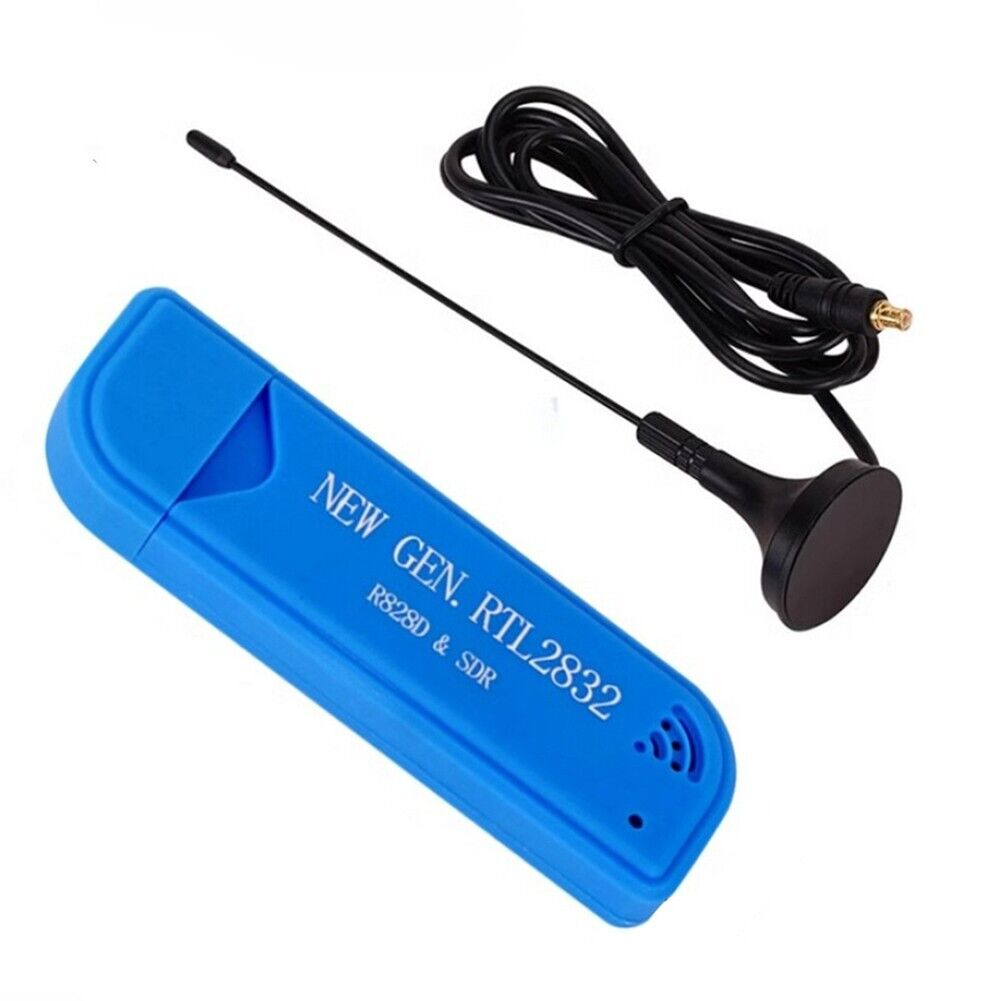
\includegraphics[width=0.3\textwidth]{rtlSdr.jpg}
    \caption{RTL-SDR with Simple SMA Antenna}
    \label{fig:rtlSDR}
\end{figure}

The RTL-SDR is based on the Realtek RTL2832U chipset, and has a frequency range of 24MHz to 1.7GHz, and a bandwidth of 3.2MHz. The RTL-SDR is also relatively cheap, with a price of around \$40 AUD. Moreover, the RTL-SDR is compatible with a wide range of software, including MATLAB, and GNU radio \cite{SDRdongle}.
The RTL-SDR was tested with a range of software as mentioned in \ref*{sec:SDRsoftware} to ensure hardware was correctly functioning and to gain familiarity with the process. Specifically, given the nature of the digital signals utilised in this project, it was tested at the appropriate frequency range (approx 200Mhz). Furthemore, this was valuable to obtain ball park noise floor measurements, which eventuated to around -80dB when using the basic antenna.

\vspace{0.5cm} \noindent 
\textbf{(ii) MODEL X Implementation}

\todo[inline]{WHAT ARE THE SPECS OF SDR X}


\subsection{Embedded Computing Platform \label{sec:embedded computing}}


\subsection{NVME Based Storage \label{sec:storage}}
Following on from the selection and testing of the Raspberry Pi 5 as the testbed computing platform, it became evident that the default 32GB microSD card used to boot and run the operating system was insufficient for the storage requirements of the project. The chosen solution for the bottleneck was to utilise a NVME SSD drive, connected via PCIe to the Raspberry Pi 5, specifically the Pimoroni Base \cite{pimoroni_nvme_base}.

In order to compare and quantify the differences in the storage performance between the microSD card and the NVME SSD, a series of tests were conducted, utilising the following linux commands via the terminal of the RPi5.

\begin{verbatim}
    lsblk
    sudo hdparm -t --direct /dev/nvme0n1 
    sudo hdparm -t --direct /dev/mmcblk0
\end{verbatim}

\noindent Resulting in the following output seen below in Table \ref{tab:diskperf}.

\begin{table}[h!]
    \centering
    \caption{Disk Read Performance: NVMe vs MicroSD Card \label{tab:diskperf}}
    \begin{tabular}{|l|l|}
    \hline
    \textbf{Device} & \textbf{Read Performance} \\ \hline
    \texttt{NVMe SSD (\texttt{/dev/nvme0n1})} & \texttt{751.22 MB/sec} \\ \hline
    \texttt{MicroSD Card (\texttt{/dev/mmcblk0})} & \texttt{84.83 MB/sec} \\ \hline
    \end{tabular}
\end{table}

The results in Table \ref{tab:diskperf} clearly show the obtained significant performance increase when using the NVME SSD compared to the microSD card. Given the large amount of data that generated and processed during the SDR sampling. Further NVME SSD configuration details include: 

\begin{itemize}
    \item \textbf{File System:} The NVME SSD was formatted with the ext4 file system, which is the default file system for most Linux distributions. 
    \item \textbf{Mounting:} The NVME SSD was mounted to the RPi5 at the following location: \texttt{/mnt/nvme}
\end{itemize}


\subsection{Antenna Configuration \label{sec:antenna}}
\subsection{Testbed Design \label{sec:testbed}}


\section{Software}
\subsection{SDR Software \label{sec:SDRsoftware}}
\subsection{Networking Requirements \label{sec:networking}}


% METHOD FOR TESTING NOT THE ACTUAL RESULTS
\section{Digital Signal Processing Testing \& Simulation}



